\documentclass[12pt, twoside]{article}
\documentclass[12pt, twoside]{article}
\usepackage[letterpaper, margin=1in, headsep=0.2in]{geometry}
\setlength{\headheight}{0.6in}
%\usepackage[english]{babel}
\usepackage[utf8]{inputenc}
\usepackage{microtype}
\usepackage{amsmath}
\usepackage{amssymb}
%\usepackage{amsfonts}
\usepackage{siunitx} %units in math. eg 20\milli\meter
\usepackage{yhmath} % for arcs, overparenth command
\usepackage{tikz} %graphics
\usetikzlibrary{quotes, angles}
\usepackage{graphicx} %consider setting \graphicspath{{images/}}
\usepackage{parskip} %no paragraph indent
\usepackage{enumitem}
\usepackage{multicol}
\usepackage{venndiagram}

\usepackage{fancyhdr}
\pagestyle{fancy}
\fancyhf{}
\renewcommand{\headrulewidth}{0pt} % disable the underline of the header
\raggedbottom
\hfuzz=2mm %suppresses overfull box warnings

\usepackage{hyperref}
\usepackage{float}

\fancyhead[LE]{\thepage}
\fancyhead[RO]{\thepage \\ First and last name: \hspace{2.5cm} \,\\ Section: \hspace{2.5cm} \,}
\fancyhead[LO]{BECA / Dr. Huson / Regents Prep: Graphs\\* 2 June 2025}

\begin{document}

\subsubsection*{3.6 Do Now: Graphing 3rd order polynomials}
\begin{enumerate}
  \item Graph the cubic function $f(x) = x^{3}-x^{2}-6x$ on the grid below. 
\begin{enumerate}
    \item Mark and label the $x$-intercepts. 
    \item Write the function in factored form. \vspace{1.5cm}
    \item Mark and label the local maximum and minimum points.
    \item Characterize the end behavior of the function. Use the notation \\
    ``as $x \rightarrow \pm \infty$ $y \rightarrow\pm \infty$"
\end{enumerate}
      \hspace{2cm}
  
    \begin{center}
    \begin{tikzpicture}[scale=.635]
      \draw [help lines] (-10,-10) grid (10,10);
      \draw [thick, ->] (-10.2,0) -- (10.4,0) node [below right] {$x$};
      \draw [thick, ->] (0,-10.2)--(0,10.4) node [left] {$y$};
      %\draw[thick, <->,smooth, domain=-3.3:2.1] plot (\x, {2.5*(\x)^2 + 3*\x - 7});
    \end{tikzpicture}
    \end{center}

\newpage

\item Find the value of each variable that makes the equation true.
\begin{multicols}{2}
\begin{enumerate}[itemsep=0.5cm]
    \item $5^2 \cdot 5^3 = 5^a \qquad a=$
    \item $\displaystyle \frac{3^7}{3^6} = 3^b \hspace{1.4cm}  b=$
    \item $7^c=1 \hspace{1.6cm} c=$
    \item $(4^3)^5 = 4^d \qquad d=$
    \item $\displaystyle 2^e = \frac{1}{2} \hspace{1.5cm}  e=$
    \item $3^4 \cdot f^4 = 15^4 \quad f=$
\end{enumerate}
\end{multicols} \vspace{0.5cm}

\item Evaluate each expression.
\begin{multicols}{2}
\begin{enumerate}[itemsep=0.5cm]
    \item $\displaystyle \frac{1}{4} \cdot 24 =$
    \item $\displaystyle \frac{3}{2} \cdot 10 =$
    \item $\displaystyle \frac{3}{5} \cdot 8 \cdot \frac{5}{3} =$
    \item $\displaystyle \frac{2}{3} \cdot \frac{5}{2} \cdot 9 =$
\end{enumerate}
\end{multicols} \vspace{0.5cm}

\item Rewrite each expression to a fractional exponent.
  \begin{multicols}{2}
    \begin{enumerate}[itemsep=1cm]
        \item $\sqrt[2]{5} =$
        \item $\displaystyle \frac{1}{\sqrt[2]{5}}=$
        \item $\sqrt[3]{5^2} =$
        \item $\displaystyle \frac{1}{(\sqrt[4]{5})^3}=$
    \end{enumerate}
    \end{multicols} \vspace{1cm}

\item Rewrite each expression with fractional exponent as a radical.
  \begin{multicols}{2}
    \begin{enumerate}[itemsep=1cm]
      \item $\displaystyle 5^{\frac{1}{3}}=$
      \item $\displaystyle 5^{-\frac{1}{2}}=$
      \item $\displaystyle 5^{\frac{3}{2}}=$
      \item $\displaystyle 5^{-\frac{5}{3}}=$
    \end{enumerate}
    \end{multicols}

\end{enumerate}
\end{document}